\section{Introduction}
Several discretization methods haven been developed for arbitrary polygonal
meshes \cite{pwld_2d,pwld_3d,pwl_diffusion,palmer_ane,palmer_proc,palmer_fe,
wachspress,cell_centered_diff,mimetic}. Polygonal cells can be advantageous 
because the number of unknowns can be reduced while maintaining symmetry 
within the mesh. This potential reduction in the number of unknowns can be 
seen by comparing a hexagonal cell with a triangular discretization of the 
same area:
\begin{figure}[H]
\centering
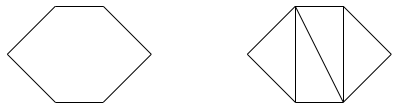
\includegraphics[width=0.5\textwidth]{hex_tri_cells}
\caption{Hexagonal cell versus triangle cells.}
\end{figure}
If there is one unknown per vertex, the hexagonal cell will have only six
unknowns compared to the twelve unknowns of the triangular discretization. 
Another advantage of polygonal cells is that they can be used for adaptive 
mesh refinement (AMR) \cite{amr_rad,amr_block,amr_unstruc} without having to
deal with hanging nodes \cite{arbitrary_hanging_nodes,dealII_hanging_nodes,
locally_hanging_nodes}. On the figure below, the left cell is a pentagon whereas 
the two cells on the right are quadrilaterals:
\begin{figure}[H]
\centering
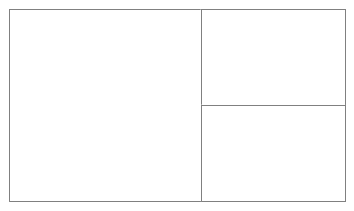
\includegraphics[width=0.3\textwidth]{amr}
\caption{AMR mesh.}
\end{figure}
Among the different discretization schemes for polygonal meshes, the PieceWise 
Linear Discontinuous (PWLD) finite elements \cite{pwld_2d,pwld_3d} have been 
successfully used to solve the transport equation. Another variant of the
PieceWise Linear finite elements, the PieceWise Linear Continuous (PWLC) finite 
elements were also developed and used to discretize the diffusion equation. 
They have shown to be second order and to produce a symmetric positive (SPD) 
matrix contrarily to others discretization for arbitrary polygonal meshes 
\cite{pwl_diffusion}. However, no Diffusion Synthetic Acceleration (DSA) 
\cite{dsa_ref,larsen_dsa,consistent_p1,mip} was developed using either PWLD or
PWLC finite elements. In this work, we will remedy this lack by adapting the 
Modified Interior Penalty (MIP) DSA developed in \cite{mip} for triangular 
cells to PWLD finite elements which will allow the DSA scheme to work on arbitrary 
polygonal cells. Since MIP produces SPD equations, it has usually 
been solved using conjugate gradient (CG) preconditioned by SSOR. In this
paper, the effectiveness of algebraic multigrid methods (AMG) to precondition 
the Krylov solver \cite{amg,amg_course} will be tested. Algebraic multigrid methods 
allow the use of multigrid techniques when there is no grid or when the mesh is 
unstructured. Instead of using a succession of grids based on the geometry of the 
problems, the grids are based on properties of the matrix.

The remainder of this paper is organized as follows. In Sec.(\ref{sec_mip}),
we introduce the PWLD finite elements and we adapt MIP to this discretization. 
In Sec.(\ref{sec_amg}), we briefly explain AMG and we introduce the two different 
AMG methods that we will use, the ML package of Trilinos \cite{ml_guide} and the 
AGMG (AGgregation-based algebraic MultiGrid) code \cite{agmg_guide}. In 
Sec.(\ref{sec_res}), we show the Fourier analysis of MIP discretized with PWLD
and we compare the different preconditioners of the CG solver. In 
Sec.(\ref{sec_conc}), we give our conclusions.
